\section*{Dati e risultati}

\subsection*{Diodo 1N4007}

Per studiare la caratteristica $I-V$ (corrente-tensione) di un diodo 1N4007 sia in polarizzazione inversa che in diretta ci siamo mossi come segue: abbiamo collegato il diodo all'alimentatore di tensione continua, misurando con il multimetro la corrente assorbita dal diodo.
Ricordiamo che durante questa prima fase dell'esperienza abbiamo prestato attenzione che la corrente attraversante il diodo non superasse i $700\,\si{\milli\ampere}$. Grazie ai dati misurati abbiamo graficato la curva caratteristica $I-V$ del diodo, mostrata in figura \ref{fig:diodo}.

\begin{SCfigure}[1][b!]
    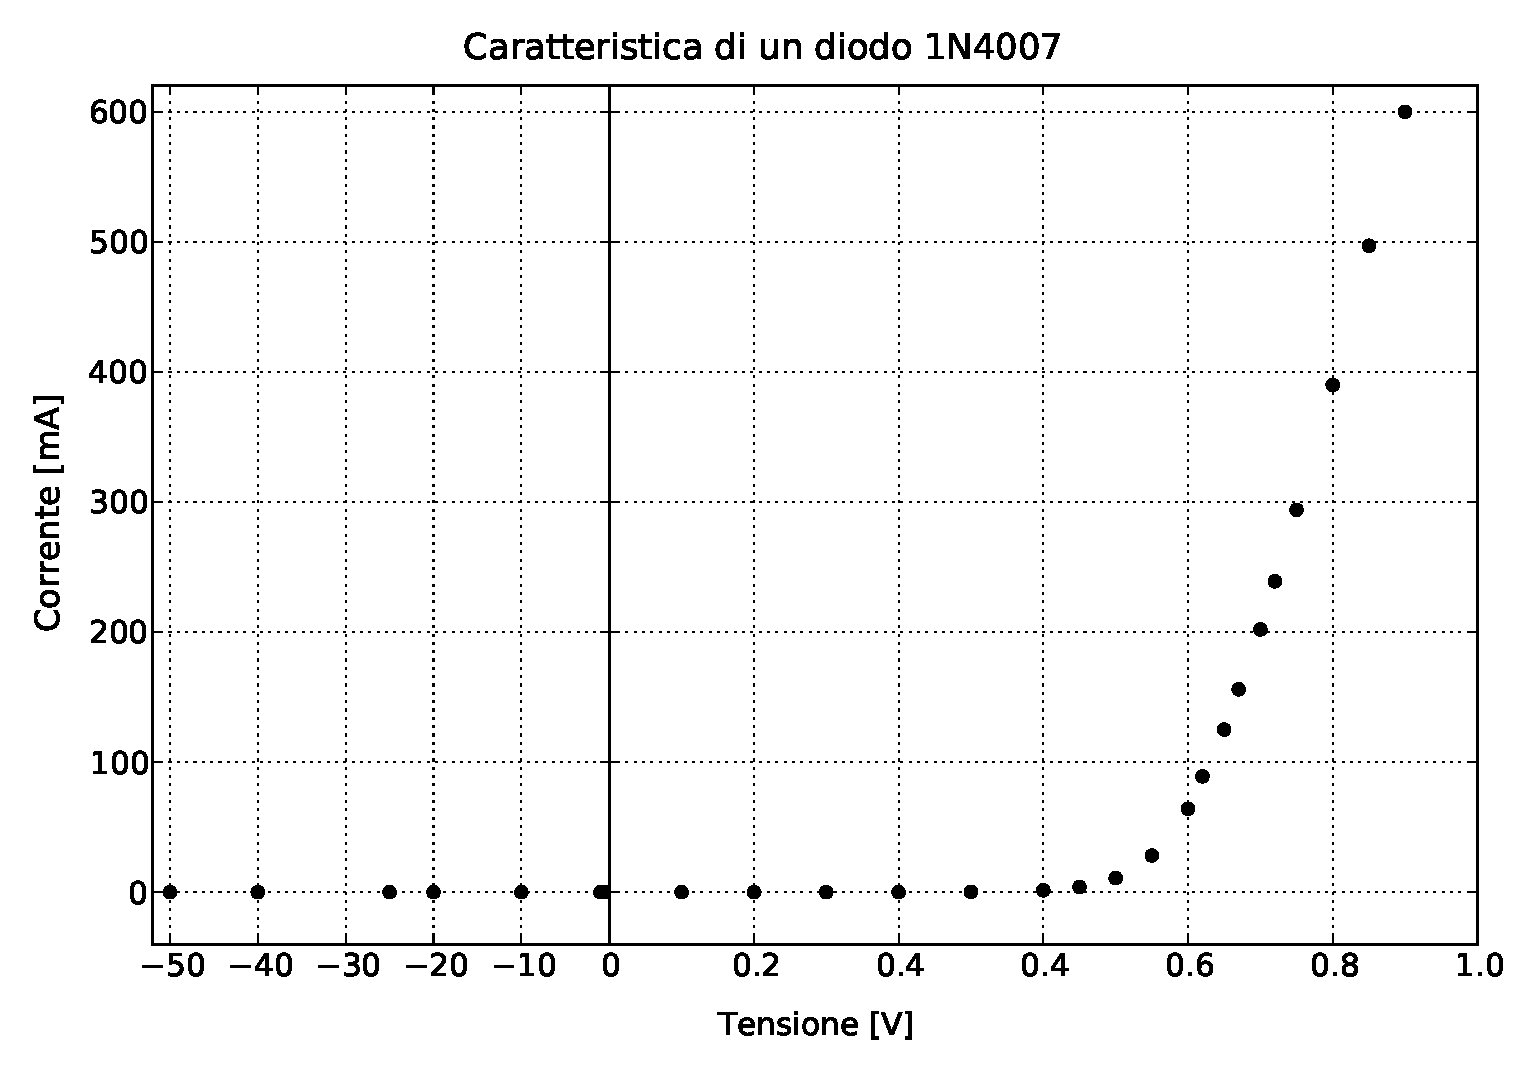
\includegraphics[scale=0.50]{diodo.pdf}
    \caption{La figura mostra la caratteristica corrente-tensione di un diodo 1N4007. Questo tipo di diodi
        ha una tensione di breakdown di circa 1000 V, valori che con il nostro alimentatore non siamo in grado di raggiungere.
        La corrente di leakage è praticamente inesistente, mentre la tensione di cut-in è di circa 0.5 V, valore vicino al valore
        tipico di 0.6 V dei diodi al silicio. }
    \label{fig:diodo}
\end{SCfigure}

\subsection*{Cella fotovoltaica}

Come secondo obbiettivo abbiamo valutato la caratteristica $I-V$ di una cella fotovoltaica al silicio. Questo andamento è stato valutato sia ponendo la cella fotovoltaica al buio, ovvero ponendola all'interno del proprio invoucro di cartone, sia esponendola ad una sorgente luminosa.
Come nel caso precedente abbiamo misurato mediante il multimetro la correte passante nella cella fotovoltaica.
Anche in questo caso abbiamo dovuto fare attenzione che la corrente massima nella cellafotovoltaica non superasse i $100\,\si{\milli\ampere}$.

\begin{SCfigure}
    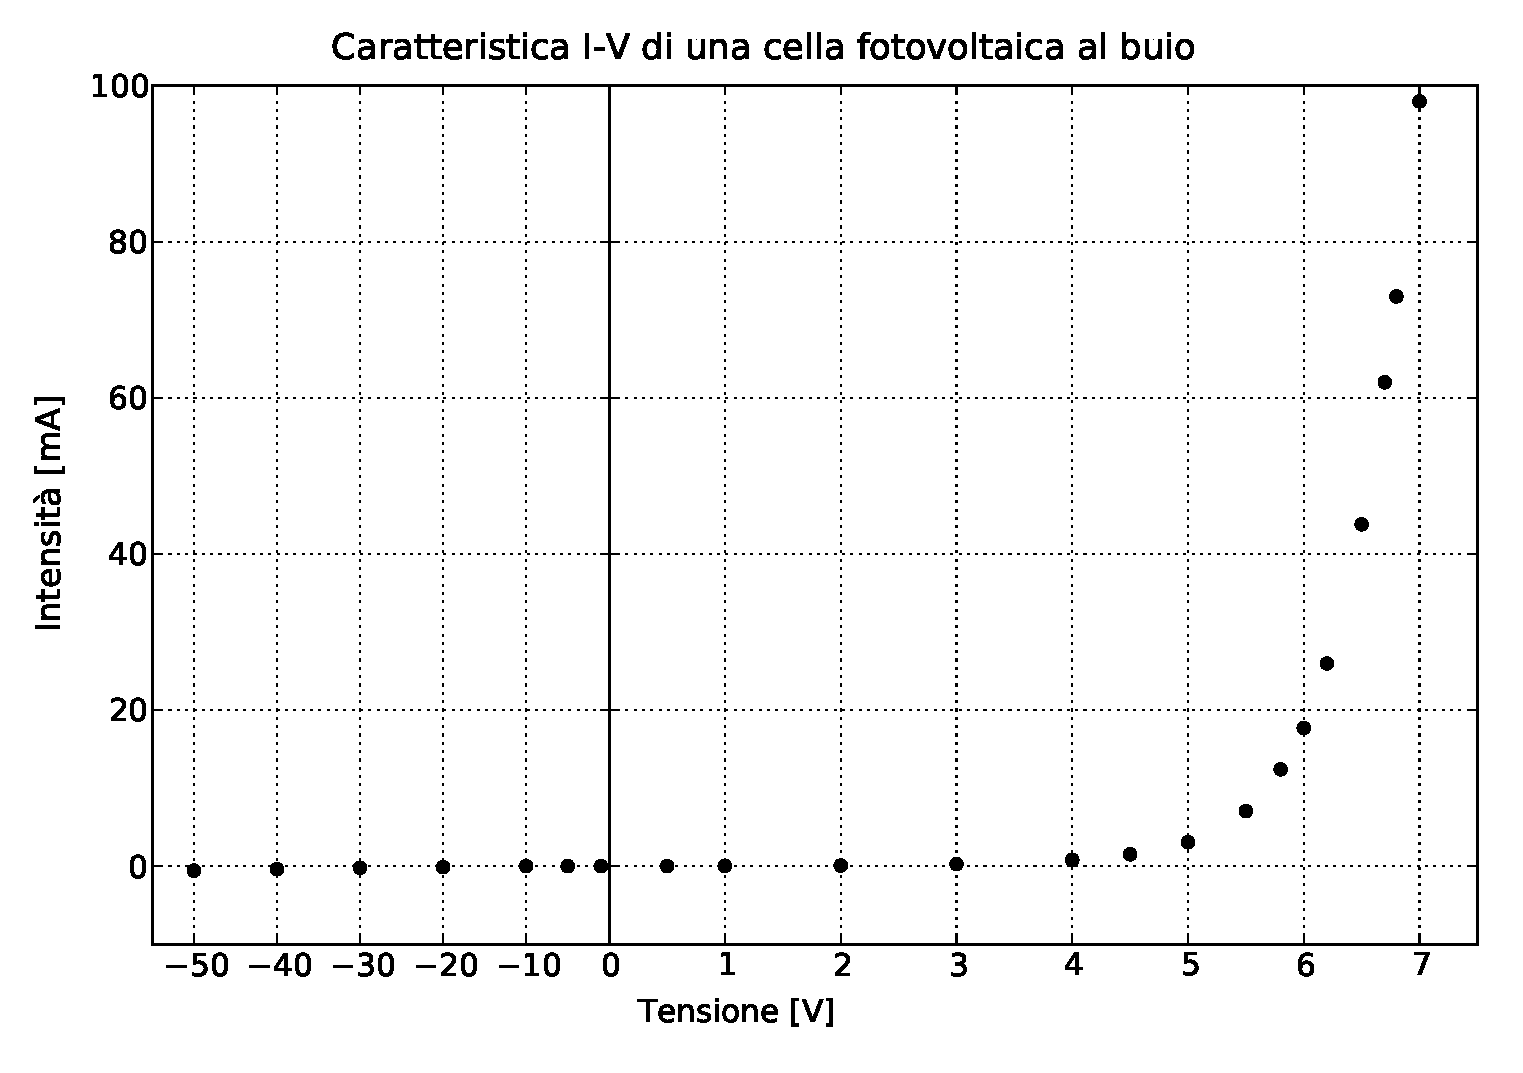
\includegraphics[scale=0.5]{buio.pdf}
    \caption{La caratteristica I-V di una cella fotovoltaica al buio è per molti aspetti simile alla caratteristica di un diodo,
        con la differenza che la tensione di attivazione è di circa 5 V.}
    \label{fig:buio}
\end{SCfigure}

\begin{SCfigure}
    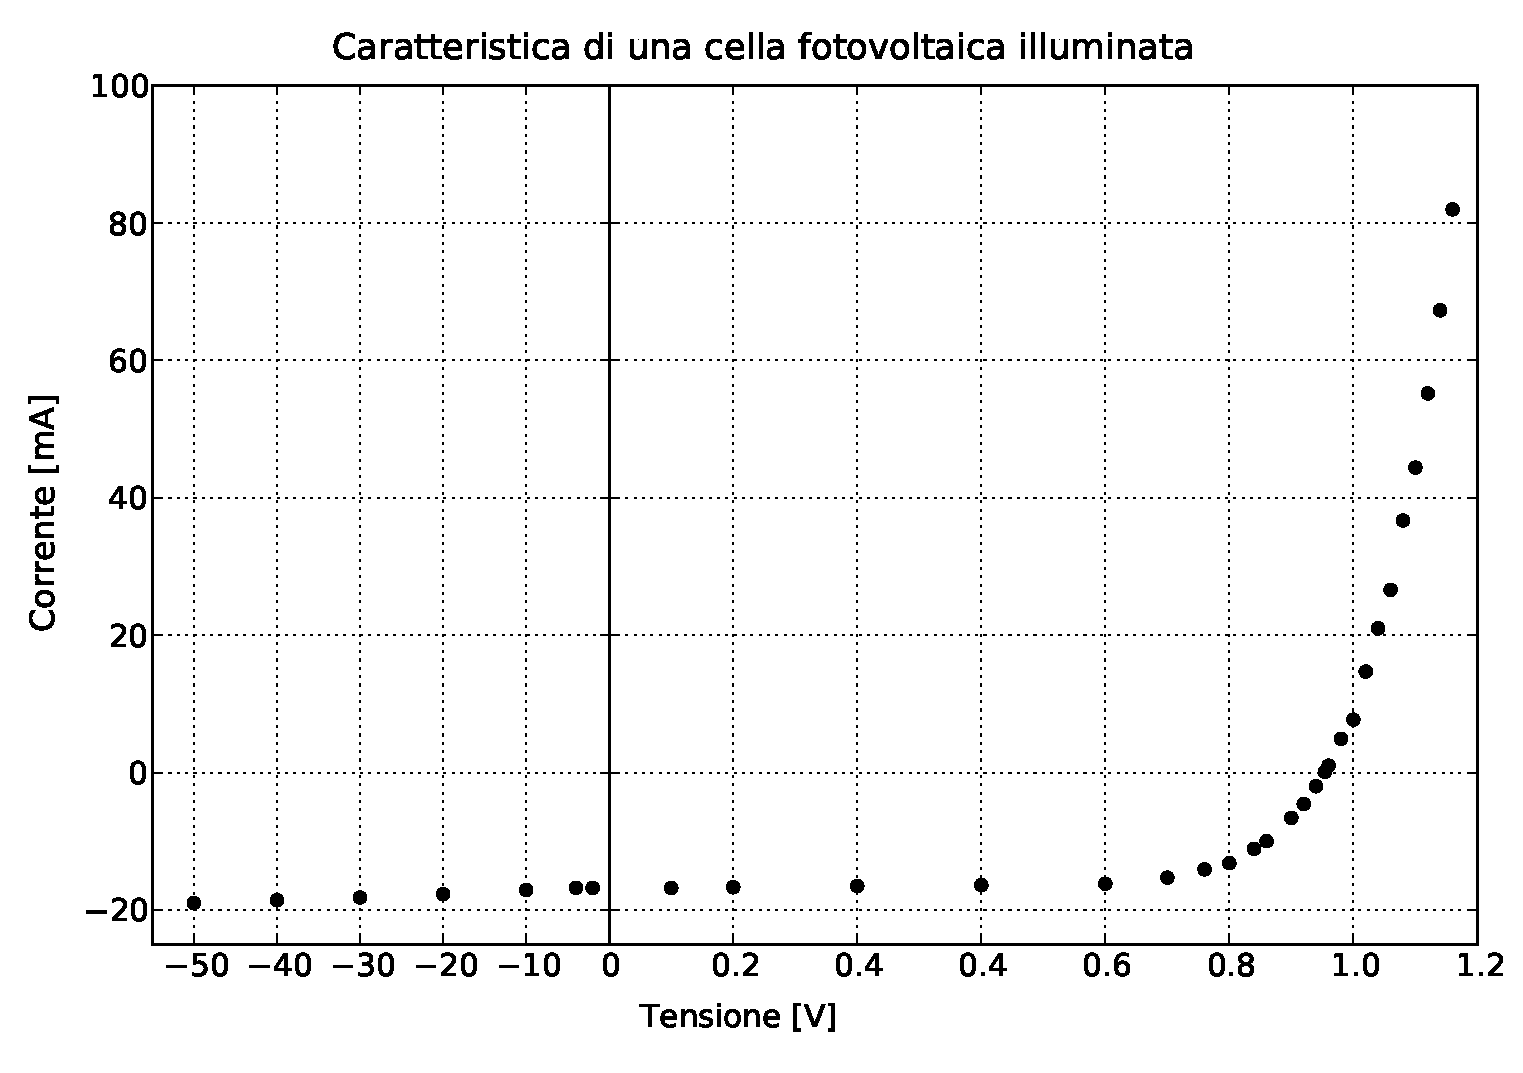
\includegraphics[scale=0.5]{luce.pdf}
    \caption{Per una cella fotovoltaica illuminata da una luce constante, la curva caratteristica varia. }
    \label{fig:luce}
\end{SCfigure}

Infine abbiamo calcolato il FillFactor, ovvero:

\subsection*{Cella fotovoltaica}

Abbiamo eseguito le stesse misure di tensione e corrente per una cella fotovoltaica monocristallina. Le misure sono state
eseguite in due configurazioni: una con la cella al buio, chiusa in una scatola, e una mantenendo una fonte di illuminazione costante
sopra di essa. I risultati sono riportati nei grafici nelle Figure \ref{fig:buio} e \ref{fig:luce}

\begin{SCfigure}
    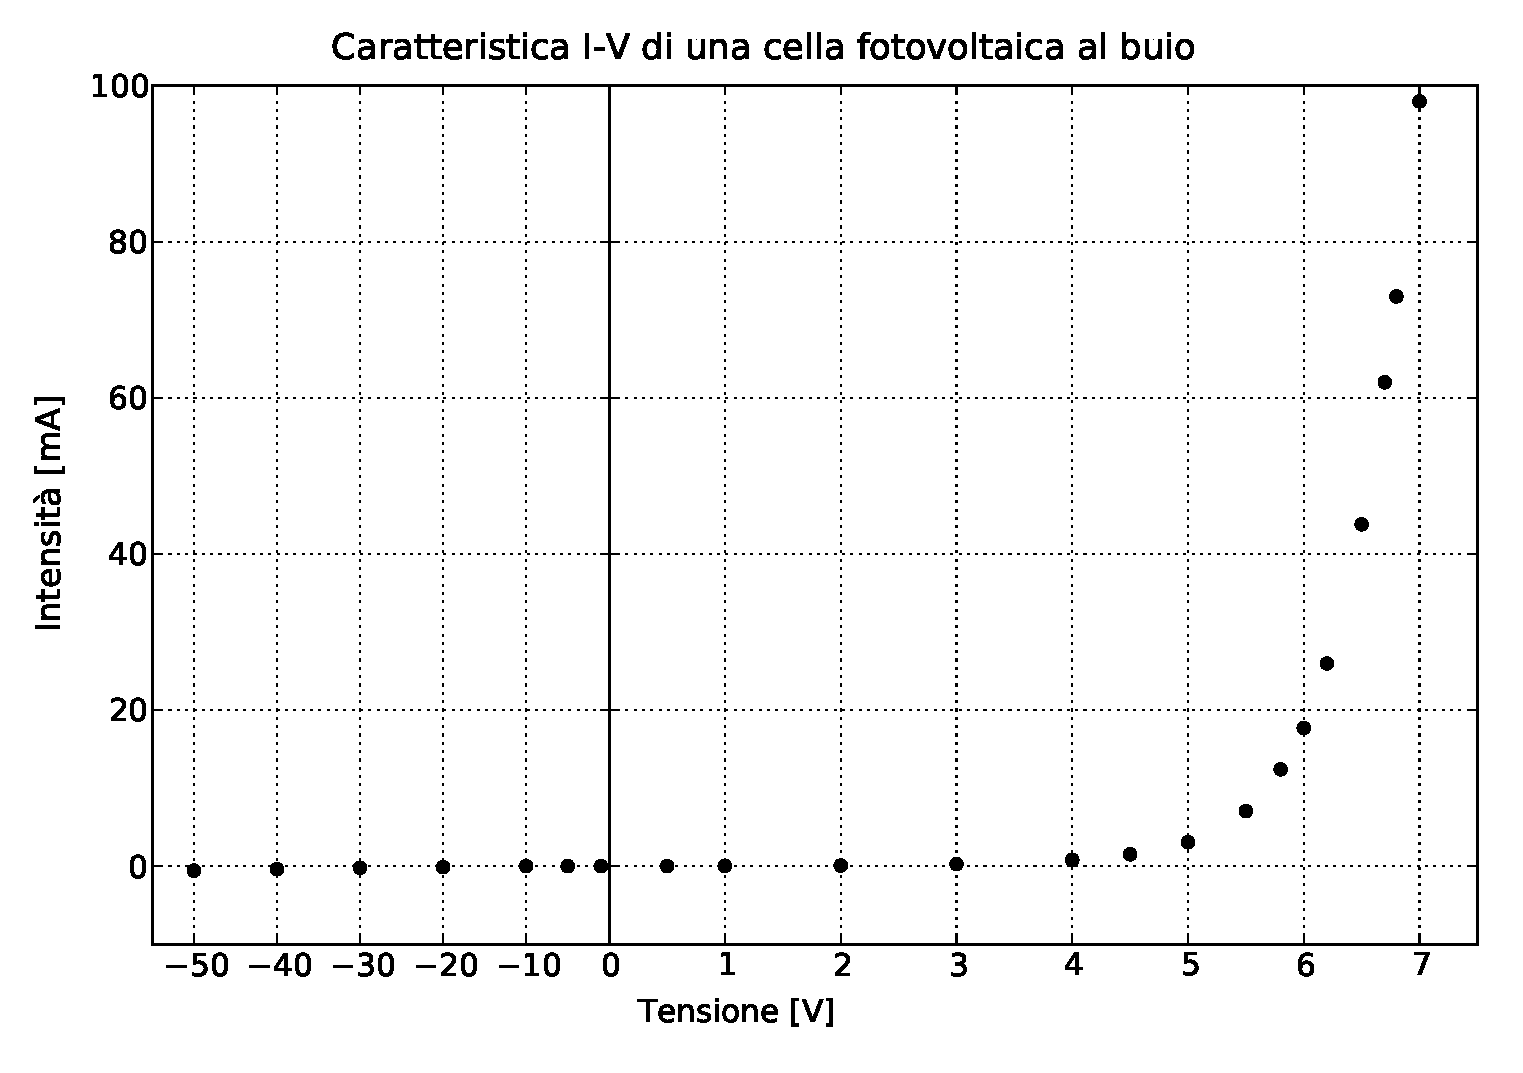
\includegraphics[scale=0.5]{buio.pdf}
    \caption{La caratteristica I-V di una cella fotovoltaica al buio è per molti aspetti simile alla caratteristica di un diodo,
        con la differenza che la tensione di attivazione è di circa 5 V.}
    \label{fig:buio}
\end{SCfigure}

\begin{SCfigure}
    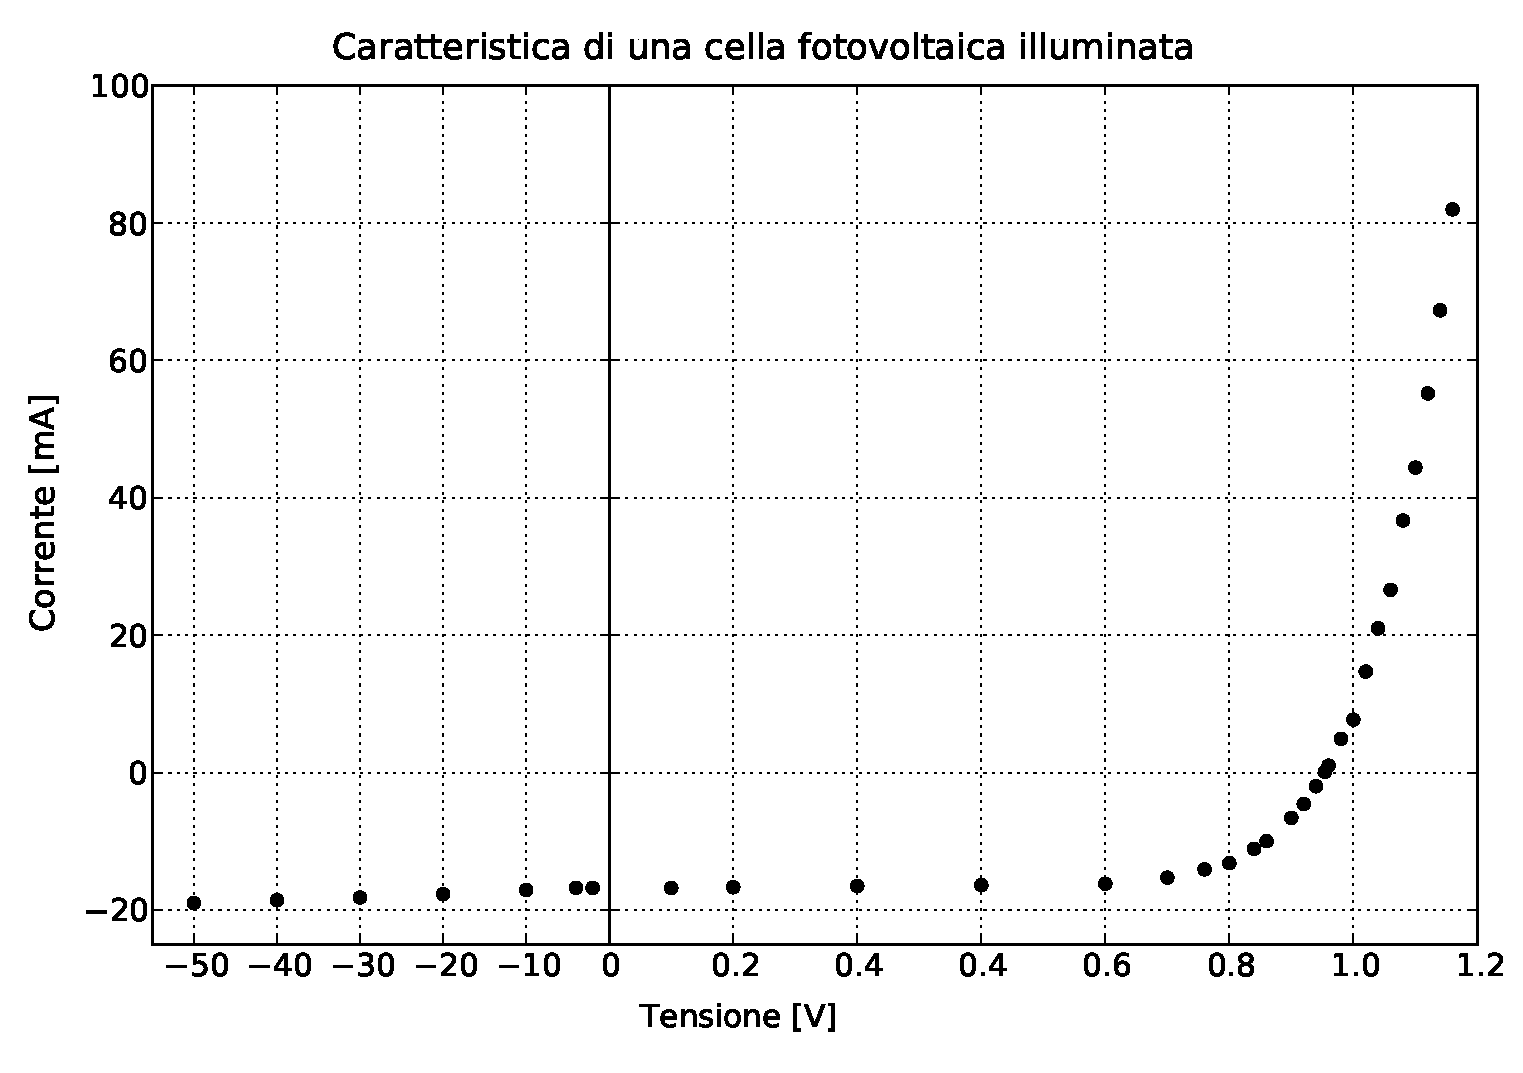
\includegraphics[scale=0.5]{luce.pdf}
    \caption{Per una cella fotovoltaica illuminata da una luce constante, la curva caratteristica varia. }
    \label{fig:luce}
\end{SCfigure}
